
%------------------2.3 温度对反应速率的影响-----------------------
\section{2.3 温度对反应速率的影响}
\begin{frame}
	\frametitle{1 阿伦尼乌斯方程}
        在幂函数型速率方程中,以温度函数$f_1(T)$来体现温度对反应速率的影响。对于一定的温度,$f_1(T)$为定值,以反应速率常数$k$来表示。通常用阿伦尼乌斯方程来表示反应速率常数与温度的关系。
    $$k = A\exp(-E/RT) $$\\
    式中,$A$为指前因子;$E$为活化能;$R$为气体常数。
    \\k的物理意义:所有反应组分的浓度均为1时的反应速率。
    \\k的单位:与反应速率的表示方式、速率方程的形式、以及反应物系组成的表示方式有关。
        \\化学反应速率总是随着温度的升高而增加(极少数者例外)。
\end{frame}


\begin{frame}
	\frametitle{2 阿伦尼乌斯方程的其他形式}
	积分式
	$$\ln{k}=\ln{A}-E/RT$$\\
	以$\ln{k}$对$1/T$作图可得一直线,由直线的斜率可决定反应的活化能。
	\\~
	\\微分式
	$$\frac{\mathrm{d}\ln{k}}{\mathrm{d}T} =\frac{E}{RT^2}$$
	\\~
	\\定积分式
	$$\ln\frac{k_2}{k_1}=\frac{-E_a}{R}(\frac{1}{T_2}-\frac{1}{T_1})$$	
\end{frame}


\begin{frame}
	\frametitle{3 正逆反应活化能的关系}
	如果可逆反应的正逆反应速率常数均符合阿伦尼乌斯方程,则有
	$$\frac{\mathrm{d}\ln\overrightarrow{k}}{\mathrm{d}T} =\frac{\overrightarrow{E}}{RT^2}~~~~~~~~
	\frac{\mathrm{d}\ln\overleftarrow{k}}{\mathrm{d}T} =\frac{\overleftarrow{E}}{RT^2}~~~~\Rightarrow ~~~~\frac{\mathrm{d}\ln\overrightarrow{k}}{\mathrm{d}T}-\frac{\mathrm{d}\ln\overleftarrow{k}}{\mathrm{d}T}=\frac{\overrightarrow{E}-\overleftarrow{E}}{RT^2}$$
	\\由正逆反应速率常数关系式$\overrightarrow{k}/\overleftarrow{k}=K_c^{1/\nu}$两边取对数,得
	$$\frac{\mathrm{d}\ln\overrightarrow{k}}{\mathrm{d}T}-\frac{\mathrm{d}\ln\overleftarrow{k}}{\mathrm{d}T}=\frac{1}{\nu}\frac{\mathrm{d}\ln{K_p}}{\mathrm{d}T}$$
	\\又有范特霍夫方程$\frac{\mathrm{d}\ln{K_p}}{\mathrm{d}T}=\frac{\Delta{H_r}}{RT^2}$,则
	$$\overrightarrow{E}-\overleftarrow{E}=\frac{1}{\nu}\Delta{H_r}$$
	\\对于吸热反应,$\Delta{H_r}>0$,所以$\overrightarrow{E}>\overleftarrow{E}$;放热反应,$\Delta{H_r}<0$,$\overrightarrow{E}<\overleftarrow{E}$;
\end{frame}


\begin{frame}
	\frametitle{4 温度对可逆反应速率的影响}
	可逆反应的反应速率等于正逆反应速率之差,用组分A的转化率$X_A$来表示可写成:
	$$r=\overrightarrow{k}f(X_A)-\overleftarrow{k}g(X_A)$$
	\\对$T$求导,得
	$$(\frac{\partial r}{\partial T} )_{X_A}=f({X_A})\frac{\mathrm{d}\overrightarrow{k}}{\mathrm{d}T}-g({X_A})\frac{\mathrm{d}\overleftarrow{k}}{\mathrm{d}T}$$
	\\根据阿伦尼乌斯方程
	$$\frac{\mathrm{d}\ln\overrightarrow{k}}{\mathrm{d}T} =\frac{\overrightarrow{E}}{RT^2}~~~~\Rightarrow~~~~\frac{\mathrm{d}\overrightarrow{k}}{\mathrm{d}T}=\frac{\overrightarrow{k}\overrightarrow{E}}{RT^2}~~~~~~~~\frac{\mathrm{d}\overleftarrow{k}}{\mathrm{d}T}=\frac{\overleftarrow{k}\overleftarrow{E}}{RT^2}$$
	$$(\frac{\partial r}{\partial T} )_{X_A}=\frac{\overrightarrow{E}}{RT^2}\overrightarrow{k}f({X_A})-\frac{\overleftarrow{E}}{RT^2}\overleftarrow{k}g({X_A})$$
\end{frame}


\begin{frame}
	\frametitle{4.1 温度对可逆吸热反应速率的影响}
			$(\frac{\partial r}{\partial T} )_{X_A}=\frac{\overrightarrow{E}}{RT^2}\overrightarrow{k}f({X_A})-\frac{\overleftarrow{E}}{RT^2}\overleftarrow{k}g({X_A})$
	\\因为$r\ge 0$,所以$\overrightarrow{k}f({X_A})\ge \overleftarrow{k}g({X_A})$。
	\\对于可逆吸热反应,$\overrightarrow{E}> \overleftarrow{E}$,$(\frac{\partial r}{\partial T} )_{X_A}> 0$
	\\可逆吸热反应的速率总是随着温度的升高而增加。
	\centerline{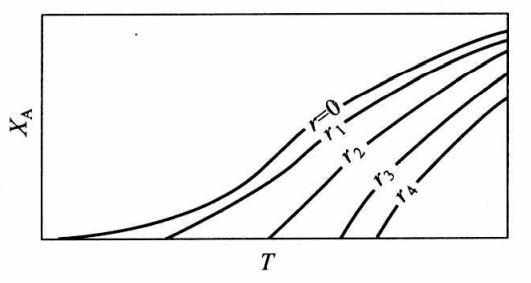
\includegraphics[height=3.8cm]{figs/fig2.2}}
	\centerline{\scriptsize{可逆吸热反应的反应速率与温度及转化率的关系($r_4>r_3>r_2>r_1$)}}
\end{frame}


\begin{frame}
	\frametitle{4.2 温度对可逆放热反应速率的影响}
	\begin{columns}[c]
	\column{7cm}
		$$(\frac{\partial r}{\partial T} )_{X_A}=\frac{\overrightarrow{E}}{RT^2}\overrightarrow{k}f({X_A})-\frac{\overleftarrow{E}}{RT^2}\overleftarrow{k}g({X_A})$$
		\\~~~~~~~~对于可逆放热反应,$\overrightarrow{E}< \overleftarrow{E}$,但$\overrightarrow{k}f({X_A})> \overleftarrow{k}g({X_A})$,所以
		\\$(\frac{\partial r}{\partial T} )_{X_A}> 0$;$(\frac{\partial r}{\partial T} )_{X_A}= 0$;$(\frac{\partial r}{\partial T} )_{X_A}< 0$
		\\~~~~~~~~可逆放热反应的速率随着温度的升高既可能增加,又可能降低,如图所示。
		\\~~~~~~~~图中曲线是在一定转化率下作出的,也叫等转化率线。
			\column{7cm}
		\centerline{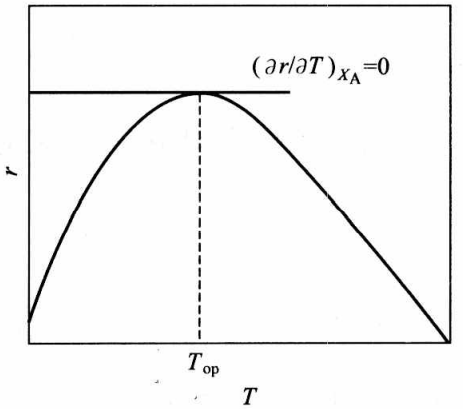
\includegraphics[height=4.5cm]{figs/fig2.3}}
		\centerline{\scriptsize{可逆放热反应的反应速率与温度的关系}}
		\\~~~~~~~~曲线的最高点$(\partial r/\partial T =0) $的温度叫做最佳温度$T_{\mathrm{op}}$。
	\end{columns}
\end{frame}


\begin{frame}
	\frametitle{4.3 可逆放热反应最佳温度曲线}
	\begin{columns}
		\column{7cm}
		反应速率极大点斜率为零,$(\frac{\partial r}{\partial T} )_{X_A}= 0$
		$$\overrightarrow{E}\overrightarrow{k}f({X_A})-\overleftarrow{E}\overleftarrow{k}g({X_A})=0$$
		$$\frac{\overrightarrow{E}\overrightarrow{A}\exp(-\overrightarrow{E}/RT_{\mathrm{op}})}{\overleftarrow{E}\overleftarrow{A}\exp(-\overleftarrow{E}/RT_{\mathrm{op}})}=\frac{g({X_A})}{f({X_A})}$$
		\\当反应达到平衡时,$$r=\overrightarrow{k}f(X_A)-\overleftarrow{k}g(X_A)=0$$
		$$\frac{g({X_A})}{f({X_A})}=\frac{\overrightarrow{k}}{\overleftarrow{k}}=\frac{\overrightarrow{A}\exp(-\overrightarrow{E}/RT_{\mathrm{e}})}{\overleftarrow{A}\exp(-\overleftarrow{E}/RT_{\mathrm{e}})}$$
				\column{7cm}
				将上式化简后两边取对数,整理后得				
		$$T_{\mathrm{op}}=\frac{T_{\mathrm{e}}}{1+\frac{RT_{\mathrm{e}}}{\overleftarrow{E}-\overrightarrow{E}}\ln\frac{\overleftarrow{E}}{\overrightarrow{E}}}$$
		\\平衡温度$T_{\mathrm{e}}$是转化率的函数,故最佳温度$T_{\mathrm{op}}$是转化率的隐函数。
		\\对应于任一转化率$X_A$,则必然有与其对应的平衡温度$T_{\mathrm{e}}$和最佳温度$T_{\mathrm{op}}$。
	\end{columns}
\end{frame}


\begin{frame}
	\frametitle{4.3 可逆放热反应最佳温度曲线}
	\begin{columns}[c]
		\column{7cm}
		\centerline{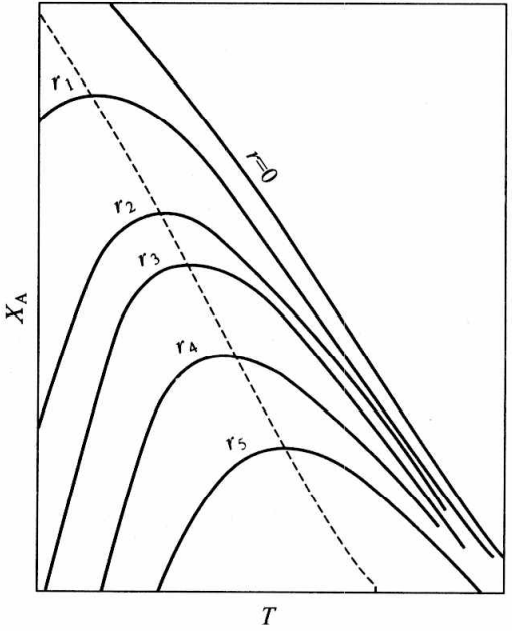
\includegraphics[width=5cm]{figs/fig2.4}}
		\centerline{\scriptsize{可逆放热反应的反应速率与温度及转化率的关系}}
		\column{7cm}
		曲线为等反应速率线,$r_5>r_4>r_3>r_2>r_1$
		\\$r=0$的曲线为平衡曲线,为反应进行的极限。
		\\连结所有等速率线上的极值点所构成的曲线(即图示虚线),叫做最佳温度曲线。
		\\对于可逆放热反应,如果从始至终按最佳温度曲线操作,那么整个过程将以最高的反应速率进行。
	\end{columns}
\end{frame}


\begin{frame}
	\frametitle{例}
	在实际生产中合成氨反应
	$$\mathrm{N_2}+1.5\mathrm{H_2}\rightleftharpoons \mathrm{NH_3}$$
	\\是在高温高压下采用熔融铁催化剂进行的。合成氨反应为可逆放热反应,故过程应尽可能按最佳温度曲线进行。现拟计算下列条件下的最佳温度:(1)在25.33MPa下,以3:1的氢氮混合气进行反应,氨含量为17\%;(2)其他条件同1,但氨含量为12\%;(3)把压力改为32.42MPa,其他条件同1。
	\\已知该催化剂的正反应活化能为$58.618×10^3\mathrm{J/mol}$,逆反应活化能为$167.48×10^3\mathrm{J/mol}$。平衡常数$K_\mathrm{p}\mathrm{(MPa^{-1})}$与温度$T$(K)及总压$p$(MPa)的关系如下:
	$$\log{K_p}=(2172.26 + 19.6478p)/T – (4.2405 + 0.02149p)$$
	
\end{frame}


